\documentclass[11pt,a4paper]{article}
\usepackage[utf8]{inputenc}
\usepackage[T1]{fontenc}

\usepackage{textcomp}
\renewcommand{\tablename}{Tabla}\renewcommand{\figurename}{Figura}
\usepackage[margin=2.2cm]{geometry}
\usepackage{booktabs}
\usepackage{array}
\usepackage{multirow}
\usepackage{amsmath,amssymb}
\usepackage{caption}
\usepackage{float}
\usepackage{graphicx}
\usepackage{xcolor}
\usepackage{hyperref}
\usepackage{enumitem}
\usepackage{needspace}
\usepackage{xspace}

\hypersetup{colorlinks=true,linkcolor=blue!60!black,urlcolor=blue!60!black}
\captionsetup{font=small,labelfont=bf}
\setlength{\parskip}{3pt}
\setlength{\parindent}{0pt}
\setlength{\emergencystretch}{3em}
\usepackage{xurl}

\DeclareRobustCommand{\sig}[1]{{\ttfamily\def\_{\textunderscore\allowbreak}#1}}
\newcommand{\um}{\,\textmu m\xspace}
\newcommand{\umd}{\,\textmu m$^2$\xspace}
\newcommand{\mmd}{\,mm$^2$\xspace}

\title{\textbf{Proyecto 3: Pochoco SoC de RTL a GDSII}\\[4pt]\Large Macro digital en GF180MCU con LibreLane}
\author{Arquitectura de Computadores \\ Universidad de los Andes \\ Semestre 2026-2 \\[6pt] \textit{Integrantes:} Nicolás Araneda \quad Vicente Calderón \quad Santiago Muñoz}
\date{Noviembre de 2026}

\begin{document}
\maketitle

Todo el código, las configuraciones y los reportes están en \url{https://github.com/nicolasaraneda/Proyecto3_Arquitectura_De_Computadores}. Los nombres de archivo, módulo y corrida son los del repositorio, y las decisiones se citan con su número en \sig{docs/decisiones.md} (D1 a D23). Las corridas usan LibreLane 3.0.16 en Docker, el PDK gf180mcuD (revisión \sig{54435919}) y la biblioteca \sig{gf180mcu\_fd\_sc\_mcu7t5v0}; el README tiene las versiones exactas, la instalación y los comandos.

La corrida final (\sig{final}, \sig{asic/rom/config.yaml}) usa $T = 100$\,ns, \sig{FP\_CORE\_UTIL} = 40\,\%, la estrategia de memoria 1 (Sección~\ref{sec:mem}), el core con lectura del banco de registros y decodificación en el fetch y el modelo de cable medido para el resizer (Sección~\ref{sec:timing}, D23). Se exige cerrar timing en las nueve esquinas que analiza LibreLane: tres de parásitos (min, nom, max) por tres de proceso, voltaje y temperatura (ss a 125\,°C y 4,5\,V, tt a 25\,°C y 5\,V, ff a $-40$\,°C y 5,5\,V). Entre ellas están la típica, \sig{nom\_tt\_025C\_5v00}, y la más lenta, \sig{max\_ss\_125C\_4v50}. LibreLane solo trata como error la típica, así que el cierre en las demás se verifica con las métricas de cada esquina (\sig{asic/verificar\_cierre.py}, D14). La Tabla~\ref{tab:cierre} resume el resultado.

\begin{table}[!htb]
\centering\small
\begin{tabular}{@{}lll@{}}
\toprule
\textbf{Criterio} & \textbf{Resultado} & \textbf{Peor esquina} \\
\midrule
DRC (Magic) & 0 violaciones & \\
DRC (KLayout, deck de GlobalFoundries) & 0 marcadores en 684 reglas & \\
LVS (Netgen) & 0 diferencias & \\
Antenas & 0 nets (1 diodo insertado) & \\
Setup: WNS y TNS & 65,73\,ns y 0\,ns & \sig{max\_ss\_125C\_4v50} \\
Hold: WNS y TNS & 0,17\,ns y 0\,ns & \sig{min\_ff\_n40C\_5v50} \\
\bottomrule
\end{tabular}
\caption{Criterios de cierre de la corrida final. El hold de \sig{nom\_ff\_n40C\_5v50} empata con el de \sig{min\_ff}. Fuente: \sig{cierre.md} y \sig{drc\_klayout/resumen.md} en \sig{asic/rom/resultados/final/}.}
\label{tab:cierre}
\end{table}

%=====================================================================
\section{Del RTL de FPGA al RTL de ASIC}
\label{sec:asic}
%=====================================================================

\sig{rtl/asic\_top.v} instancia \sig{pochoco\_soc} sin nada propio de la Go Board. Sus puertos son \sig{clk}, \sig{rst\_n} (activo en bajo), \sig{btn[3:0]}, \sig{led[3:0]}, \sig{seg1[6:0]} y \sig{seg2[6:0]} (un display cada uno, en orden \{G,F,E,D,C,B,A\} y activos en alto) y \sig{spi\_sclk}, \sig{spi\_mosi}, \sig{spi\_cs\_n} y \sig{spi\_miso}. El reset pasa por un sincronizador de dos flip-flops que lo activa en forma asíncrona y lo libera en un flanco de reloj, así que todos los flip-flops salen del reset en el mismo ciclo (D6). Los parámetros \sig{MemStrategy} y \sig{DataWords} eligen la memoria de la Sección~\ref{sec:mem}, y \sig{EarlyRead} la temporización del core (Sección~\ref{sec:rtl}).

Para encontrar lo que dependía de la FPGA se corrió LibreLane sobre el RTL del Proyecto 2 (commit \sig{1227fa5}) aplicando los reemplazos de a uno: c0a con el RTL sin cambios, c0b con el banco de registros en flip-flops y c0c con \sig{asic\_top}. La Tabla~\ref{tab:fpga} lista cada construcción con el mensaje del flujo que la evidenció.

\begin{table}[!htb]
\centering\small
\begin{tabular}{@{}p{3.6cm}p{6.4cm}p{5.6cm}@{}}
\toprule
\textbf{Construcción} & \textbf{Mensaje del flujo (archivo:línea)} & \textbf{Reemplazo} \\
\midrule
BRAM \sig{SB\_RAM40\_4K} en \sig{espino\_register\_file.v} & \sig{\%Error-MODMISSING ... SB\_RAM40\_4K}, el linter detiene el flujo (\sig{c0a-verilator-lint.txt:1} y \sig{:13}) & Banco de registros en flip-flops con lectura sincrónica, igual que la BRAM (D3, D4) \\
\addlinespace
Contador de reset de encendido \sig{por\_cnt} con valor inicial & \sig{\%Warning-PROCASSINIT ... 'por\_cnt'} (\sig{c0b/verilator-lint.txt:7}) y \sig{Set init value: \textbackslash por\_cnt} (\sig{c0b/yosys-synthesis.txt:324}) & Puerto \sig{rst\_n} con sincronizador en \sig{asic\_top} (D6) \\
\addlinespace
\sig{\$readmemh} dentro de un \sig{initial} (\sig{pochoco\_ram.v:36}) & \sig{Removed top 23 address bits ... from memory init port} (\sig{c0b/yosys-synthesis.txt:992}): Yosys lo convierte en valor inicial de la memoria & ROM y memoria generadas por el assembler (Sección~\ref{sec:mem}) \\
\addlinespace
Inferencia de BRAM para la RAM de 512 palabras & \sig{Adding EN signal on \$memory\textbackslash u\_soc.u\_ram.mem[93]} (\sig{c0b/yosys-synthesis.txt:1469}): la memoria pasa a flip-flops; \sig{c0b/stat.rpt}: 17\,188 flip-flops y 2\,327\,825\umd & Memoria dimensionada según el uso del juego (Sección~\ref{sec:mem}) \\
\addlinespace
SPI sin instanciar & \sig{\%Warning-UNUSEDSIGNAL ... 'spi\_req'} (\sig{c0b/verilator-lint.txt:18}) & Puertos presentes, \sig{spi\_miso} fijo en 1: el juego no usa SPI (D7) \\
\bottomrule
\end{tabular}
\caption{Construcciones del Proyecto 2 que dependían de la FPGA. Los archivos son copias de los logs de LibreLane en \sig{asic/p2\_original/evidencia/}.}
\label{tab:fpga}
\end{table}

Los dos valores iniciales son el problema de fondo. La biblioteca no tiene flip-flops con valor de encendido, así que la síntesis los descarta sin otro aviso que esas líneas. En silicio \sig{por\_cnt} partiría en un valor cualquiera, con un reset interno de entre 0 y 4095 ciclos, y la RAM partiría con instrucciones arbitrarias. Cuatro construcciones no produjeron ningún mensaje porque son valores o convenciones, no sintaxis:

\begin{itemize}[nosep,leftmargin=1.2em]
\item \sig{x0} valía 0 solo porque la BRAM se inicializaba en cero y nunca se escribía. En el banco nuevo \sig{x0} no se almacena, la lectura de la dirección 0 entrega 0 por hardware y el write-through de la Sección~\ref{sec:rtl} tampoco lo adelanta.
\item Los segmentos salían invertidos (\sig{\textasciitilde seg1}) porque el display de la Go Board es activo en bajo. En el macro los puertos quedan activos en alto, que es la función lógica (D8).
\item \sig{CYCLES\_PER\_TENTH = 2500000} en \sig{game.s} supone el oscilador de 25\,MHz de la placa. Se corrige para el macro en la Sección~\ref{sec:constantes}.
\item \sig{DebounceDivBits = 15} se eligió para 25\,MHz. A 10\,MHz da una muestra cada 3,3\,ms y acepta un cambio en unos 10\,ms, muy por debajo de la décima que muestra el juego, así que se mantuvo (D10).
\end{itemize}

%=====================================================================
\section{Memoria y programa del juego}
\label{sec:mem}
%=====================================================================

El juego usa 115 palabras de instrucciones (460 bytes) y 0 de datos. Las 115 las cuenta el assembler al ensamblar \sig{sw/game.s}: lo informa al terminar y queda como \sig{GAME\_WORDS} en la imagen generada. Las 0 de datos salen del programa y de la simulación: todos los \sig{lw} y \sig{sw} usan como base \sig{x2}, que apunta a los periféricos en \sig{0x8000\_0000}, y la simulación de la partida completa (\sig{tb/game\_tb.v}) no hace ninguna lectura ni escritura en la memoria. Las dos cantidades quedan bajo el máximo recomendado de 256 y 64. Se dejó una RAM de datos de 4 palabras en ambas estrategias (D9): conserva la RAM que nombra la estrategia 1 por 128 flip-flops, y con el mismo valor en las dos la comparación mide solo cómo se guarda el programa.

\textbf{Extensión del assembler.} Se agregaron dos salidas Verilog. \sig{--rom} escribe el módulo \sig{rtl/gen/pochoco\_rom.v} completo: un \sig{case} con una palabra por dirección, comentada con su desensamblado, sin reloj ni flip-flops, que entrega 0 fuera del programa. \sig{--vh} escribe \sig{rtl/gen/game\_image.vh} con \sig{GAME\_WORDS} y la función \sig{game\_word(i)}. \sig{make image} regenera ambos desde \sig{game.s}, y siete pruebas nuevas (\sig{assembler/tests/test\_image.py}, 80 en total) comprueban que coinciden con el \sig{.hex} y con el \sig{game.s} actual.

\textbf{Estrategias.} En la estrategia 1 (\sig{rtl/pochoco\_mem\_rom.v}) la ROM entrega la instrucción por dos salidas: una registrada, que conserva la lectura registrada de la RAM del Proyecto 2, y una combinacional (\sig{a\_next\_o}), con la que el core lee el banco de registros y decodifica un ciclo antes (Sección~\ref{sec:rtl}). El puerto de datos ve la RAM de 4 palabras en flip-flops. En la estrategia 2 (\sig{rtl/pochoco\_mem\_ff.v}) instrucciones y datos comparten una memoria de $115 + 4 = 119$ palabras en flip-flops, y el programa entra como valor de reset: cada bit queda como un flip-flop con reset o con set según la imagen, y cualquier palabra se puede escribir desde el puerto de datos, como en el Proyecto 2. Con esta memoria el core usa la temporización anterior, con un ciclo de espera por instrucción (\sig{EarlyRead = 0}). La Tabla~\ref{tab:estrategias} compara las dos con el RTL y la configuración del flujo de la corrida final.

\begin{table}[!htb]
\centering\small
\begin{tabular}{@{}lrr@{}}
\toprule
 & \textbf{Estrategia 1 (ROM)} & \textbf{Estrategia 2 (flip-flops)} \\
\midrule
Área de celdas de síntesis & 156\,098\umd & 696\,640\umd \\
Área de celdas tras place and route & 208\,439\umd & 977\,015\umd \\
Flip-flops & 964 & 4\,673 \\
Utilización real (pedida: 40\,\%) & 53,5\,\% & 56,2\,\% \\
Área del die & 0,419\mmd & 1,802\mmd \\
Período mínimo que cierra timing & 21,5\,ns & $\leq 32$\,ns \\
Frecuencia máxima & 46,51\,MHz & $\geq 31{,}25$\,MHz \\
CPI del juego completo & 1,665 & 2,665 \\
MIPS ($f/\text{CPI}$) & 27,9 & $\geq 11{,}7$ \\
Nets con violación de antena & 0 & 0 \\
\bottomrule
\end{tabular}
\caption{Estrategias de memoria a $T = 100$\,ns (corridas \sig{final} y \sig{s4\_t100}) y período mínimo de sus barridos (\sig{f2\_*}, con pasos de 0,5\,ns cerca del límite, y \sig{s4\_*}). En la estrategia 2, 32\,ns es el menor período medido: la corrida de 30\,ns no termina dentro de los 40 minutos que se fijaron por corrida. Fuente: \sig{docs/datos\_informe.md}, sección 3.2.}
\label{tab:estrategias}
\end{table}

La estrategia 2 tiene 3\,709 flip-flops más, casi todos de los $119 \times 32 = 3\,808$ bits de su memoria unificada. La ROM guarda los mismos $115 \times 32$ bits como lógica combinacional y ocupa 7\,448\umd, el 4,5\,\% del diseño (Sección~\ref{sec:sintesis}). La ruta crítica de la estrategia 2 (\sig{s4\_t32}) parte del mismo registro de decodificación y cruza la misma ALU que la de la estrategia 1 (Sección~\ref{sec:ruta}), pero desde la dirección calculada (\sig{lsu\_addr[4]}) sigue por 31 celdas y 17,4\,ns de lógica aplanada hasta \sig{\_33833\_}, un flip-flop con reset; en la estrategia 1 ese último tramo toma 4,4\,ns. La ROM combinacional es además la que aprovecha el pipeline de la corrida final. La memoria en flip-flops también tiene esa salida, pero sale del multiplexor de 119 palabras, que quedaría en el camino de la lectura anticipada; como la estrategia 2 no es la de la corrida final, se dejó con el ciclo de espera, lo que además mantiene probado el camino anterior del core. Se eligió la estrategia 1 por área y frecuencia (D17), y con el pipeline rinde además 2,4 veces los MIPS medidos de la 2 en un die 4,3 veces menor.

%=====================================================================
\section{Síntesis}
\label{sec:sintesis}
%=====================================================================

La corrida final aplana el diseño salvo el register file, la ALU y el contador de ciclos, cuya jerarquía conserva con \sig{SYNTH\_KEEP\_HIERARCHY\_MODULES} (D12). El contador se separó en su propio módulo, \sig{pochoco\_cycle\_counter}, con el mismo comportamiento. Para repartir el área entre todos los módulos se sintetizó además la misma configuración sin aplanar (\sig{SYNTH\_HIERARCHY\_MODE=keep}, corrida \sig{h3\_t100}, solo hasta Yosys), cuyo reporte separa cada módulo. Las dos síntesis difieren solo en que la aplanada optimiza a través de los bordes de módulo, y por eso su área es 5,2\,\% menor (156\,098 contra 164\,605\umd).

\begin{table}[!htb]
\centering\small
\begin{tabular}{@{}lrrp{9.6cm}@{}}
\toprule
\textbf{Celda} & \textbf{Cant.} & \textbf{\%} & \textbf{Qué parte del diseño la explica} \\
\midrule
\sig{nand2\_1} & 934 & 16,7 & NAND de dos entradas, una de las celdas más chicas de la biblioteca (11\umd). Yosys, con la estrategia de área, mapea sobre ella la lógica aleatoria: 265 en el register file, 106 en la ALU, 85 en la LSU, 79 en la etapa ID y 74 en la ROM. \\
\addlinespace
\sig{mux2\_2} & 889 & 15,9 & Multiplexor 2:1. La biblioteca no tiene flip-flops con habilitación, así que cada bit que se escribe bajo condición lleva un mux de retención delante. El banco de registros tiene 796: los 480 de retención de sus bits y el resto en los dos puertos de lectura, donde entran el write-through y la habilitación de lectura. Otros 160 son de la memoria y 117 de la etapa ID (retención del decode registrado y muxes de operandos). \\
\addlinespace
\sig{dffq\_1} & 779 & 14,0 & Flip-flop sin reset. 544 son del banco de registros ($15 \times 32 = 480$ bits más los dos puertos de lectura registrados, 64), 192 de la memoria (registro de instrucción, RAM de 4 palabras y salida de datos), 82 del decode registrado y 2 del offset de byte de la LSU. La síntesis aplanada elimina 41, entre ellos 28 bits del registro de instrucción que el core ya no lee. \\
\addlinespace
\sig{aoi21\_1} & 437 & 7,8 & Lógica aleatoria: 190 en el register file, 53 en la ALU, 48 en la ROM y 40 en la etapa ID. \\
\addlinespace
\sig{oai21\_1} & 348 & 6,2 & Lógica aleatoria: 64 en el register file, 49 en la ROM, 48 en la etapa ID y 47 en la ALU. \\
\bottomrule
\end{tabular}
\caption{Las cinco celdas más usadas de la corrida final (5\,577 celdas de 36 tipos). El reparto por módulo sale de la síntesis jerárquica \sig{h3\_t100}, que tiene más celdas porque no optimiza a través de los bordes de módulo. Fuente: \sig{asic/sintesis.md}.}
\label{tab:celdas}
\end{table}

\begin{table}[!htb]
\centering\small
\begin{tabular}{@{}llrr@{}}
\toprule
\textbf{Módulo} & \textbf{Instancia} & \textbf{Área (\textmu m$^2$)} & \textbf{\%} \\
\midrule
\sig{espino\_register\_file} & \sig{u\_soc.u\_core.u\_rf} & 80\,349 & 48,8 \\
\sig{espino\_id\_stage} (con ALU y decodificador) & \sig{u\_soc.u\_core.u\_id} & 29\,589 & 18,0 \\
\quad \sig{espino\_alu} & \sig{u\_soc.u\_core.u\_id.u\_alu} & 10\,153 & 6,2 \\
\sig{pochoco\_mem\_rom} (con la ROM) & \sig{u\_soc.g\_mem\_rom.u\_mem} & 27\,458 & 16,7 \\
\quad \sig{pochoco\_rom} & \sig{u\_soc.g\_mem\_rom.u\_mem.u\_rom} & 7\,448 & 4,5 \\
\sig{pochoco\_periph} (con debounce y contador) & \sig{u\_soc.u\_periph} & 14\,409 & 8,8 \\
\quad \sig{pochoco\_cycle\_counter} & \sig{u\_soc.u\_periph.u\_cycles} & 3\,943 & 2,4 \\
\sig{espino\_if\_stage} & \sig{u\_soc.u\_core.u\_if} & 8\,511 & 5,2 \\
\sig{espino\_load\_store\_unit} & \sig{u\_soc.u\_core.u\_lsu} & 2\,819 & 1,7 \\
Bus, sincronizador de reset y control & & 1\,470 & 0,9 \\
\midrule
\textbf{Total} & & \textbf{164\,605} & \textbf{100} \\
\bottomrule
\end{tabular}
\caption{Área de celdas por módulo en la síntesis jerárquica \sig{h3\_t100}. Las filas con sangría están incluidas en la de arriba. Fuente: \sig{asic/sintesis.md}.}
\label{tab:modulos}
\end{table}

El módulo con más área es el register file (Tabla~\ref{tab:modulos}), con 80\,349\umd: 48,8\,\% de la síntesis jerárquica y 51,5\,\% de la final, donde conserva su jerarquía y mide lo mismo. El contador de ciclos ocupa 3\,943\umd, el 2,4\,\% de la síntesis jerárquica y el 2,5\,\% de la final; el 61\,\% de su área son sus 32 flip-flops con reset y el resto el incrementador.

Antes de sintetizar se esperaba que el banco de registros dominara el área (480 bits sin celdas de memoria en la biblioteca y dos árboles de lectura de 15 a 1) y que los flip-flops fueran la celda más numerosa. Lo primero se cumple; lo segundo no: \sig{dffq\_1} queda tercera, detrás de \sig{nand2\_1} y \sig{mux2\_2} (Tabla~\ref{tab:celdas}). El conteo de flip-flops sí coincide con el RTL: 820 sin reset y 185 con reset en la síntesis jerárquica, 964 en la final. La diferencia está en la lógica del banco: con el write-through y la habilitación de lectura del pipeline (Sección~\ref{sec:rtl}) pasa de 88 a 265 \sig{nand2\_1} respecto del banco sin pipeline, y de 622 a 796 \sig{mux2\_2}, en parte por esa lógica y en parte porque la síntesis rehízo el árbol de lectura con menos \sig{mux4\_1} (de 128 a 66). Tampoco se esperaba el peso de los multiplexores: casi un \sig{mux2\_2} por flip-flop escrito bajo condición, porque la biblioteca no tiene flip-flops con habilitación.

%=====================================================================
\section{Timing}
\label{sec:timing}
%=====================================================================

\subsection{Barrido de período}

La Tabla~\ref{tab:barrido} barre \sig{CLOCK\_PERIOD} con el RTL y la configuración de la corrida final, con pasos de 0,5\,ns cerca del límite. El diseño cierra hasta 21,5\,ns y no a 21\,ns, donde falla por 0,129\,ns en la esquina lenta. La frecuencia máxima es 46,51\,MHz. El rendimiento se mide con la Ley de Hierro: tiempo $=$ instrucciones $\times$ CPI $\times T$, o sea MIPS $= f/\text{CPI}$; con el CPI de 1,665 del juego completo, la corrida final rinde 27,9\,MIPS.

\begin{table}[!htb]
\centering\footnotesize
\setlength{\tabcolsep}{4pt}
\begin{tabular}{@{}r rrrr rrrr r c@{}}
\toprule
 & \multicolumn{4}{c}{\textbf{Setup (ns)}} & \multicolumn{4}{c}{\textbf{Hold (ns)}} & & \\
\cmidrule(lr){2-5}\cmidrule(lr){6-9}
 & \multicolumn{2}{c}{\sig{nom\_tt}} & \multicolumn{2}{c}{\sig{max\_ss}} & \multicolumn{2}{c}{\sig{nom\_tt}} & \multicolumn{2}{c}{\sig{max\_ss}} & \textbf{Área} & \textbf{Cierra} \\
\textbf{T (ns)} & WNS & TNS & WNS & TNS & WNS & TNS & WNS & TNS & \textbf{(\textmu m$^2$)} & \textbf{(9 esq.)} \\
\midrule
100 & 74,404 & 0 & 65,725 & 0 & 0,442 & 0 & 1,065 & 0 & 208\,439 & sí \\
30 & 16,460 & 0 & 4,924 & 0 & 0,442 & 0 & 1,065 & 0 & 219\,059 & sí \\
25 & 12,306 & 0 & 1,579 & 0 & 0,442 & 0 & 1,065 & 0 & 219\,531 & sí \\
24 & 11,931 & 0 & 1,755 & 0 & 0,442 & 0 & 1,065 & 0 & 220\,655 & sí \\
23 & 11,272 & 0 & 1,494 & 0 & 0,442 & 0 & 1,065 & 0 & 222\,714 & sí \\
22 & 10,358 & 0 & 0,656 & 0 & 0,442 & 0 & 1,065 & 0 & 224\,767 & sí \\
21,5 & 10,257 & 0 & 0,876 & 0 & 0,442 & 0 & 1,065 & 0 & 231\,229 & sí \\
21 & 9,614 & 0 & $-0{,}129$ & $-0{,}291$ & 0,442 & 0 & 1,065 & 0 & 231\,638 & no \\
\bottomrule
\end{tabular}
\caption{Barrido de \sig{CLOCK\_PERIOD} (corridas \sig{final} y \sig{f2\_*}) en la esquina típica \sig{nom\_tt\_025C\_5v00} y la más lenta \sig{max\_ss\_125C\_4v50}. El área es la de celdas estándar tras place and route. Fuente: \sig{metrics.json} y \sig{cierre.md} de cada corrida en \sig{asic/rom/resultados/}.}
\label{tab:barrido}
\end{table}

Cada \sig{CLOCK\_PERIOD} puede provocar una nueva optimización del circuito: el resizer cambia el tamaño de las celdas y agrega buffers según el período, y eso cambia el área, el buffering y el placement. Aquí el área de celdas sube en cada punto, de 208\,439\umd a 100\,ns a 231\,229\umd a 21,5\,ns (11\,\% más), y por eso el WNS no baja un nanosegundo por cada nanosegundo de período: es 1,755\,ns a 24\,ns, más que a 25\,ns, y 0,876\,ns a 21,5\,ns, más que a 22\,ns. El barrido termina porque el diseño deja de cerrar, no porque el resizer deje de encontrar qué mejorar. El hold no depende del período y es el mismo en los ocho puntos.

El límite también depende de la configuración del flujo. Con la del PDK, el resizer usaba celdas de retardo (\sig{dly*}) como buffers, 12 de ellas en la ruta crítica a 60\,ns, y se excluyeron (D15); se excluyó además \sig{buf\_1} y se le pidió un margen de setup de 10\,ns (D20). El cambio mayor vino de medir cuánto se equivoca el resizer con los cables. Durante el placement y el CTS estima los parásitos con el promedio de las capas del tech LEF, 0,2752\,$\Omega$/\textmu m y 64,3\,aF/\textmu m en las nueve esquinas. Una regresión lineal de la resistencia y la capacidad que extrae OpenRCX contra el largo ruteado, sobre los 2\,399 nets de más de 20\um de una corrida, da entre 0,498 y 0,599\,$\Omega$/\textmu m y entre 148,0 y 188,4\,aF/\textmu m según la extracción (min a max): el resizer subestimaba la capacidad de los cables entre 2,3 y 2,9 veces y su resistencia entre 1,8 y 2,2 veces (\sig{asic/modelo\_cable.py}, \sig{docs/modelo\_cable.md}).

Con parásitos de menos daba un net por cumplido sin poner el buffer, y la violación aparecía recién en el STA final; por eso la corrida final anterior tenía 546 pines con violación de max slew. La corrida final reemplaza esa tabla por los valores del tech LEF multiplicados, capa por capa, por el factor medido en cada extracción (\sig{LAYERS\_RC}), y repite la reparación de slew, capacitancia y timing después del ruteo global (\sig{RUN\_POST\_GRT\_DESIGN\_REPAIR} y \sig{RUN\_POST\_GRT\_RESIZER\_TIMING}). Así quedan 0 violaciones de max slew en las nueve esquinas, a 100 y a 21,5\,ns, y una de max capacitancia en la raíz del árbol de reloj (0,43\,pF contra el límite de 0,2\,pF del flujo; la biblioteca admite 3,93\,pF en ese pin), un pin que la reparación no modifica.

\subsection{Ruta crítica}
\label{sec:ruta}

La ruta crítica a 21,5\,ns en la esquina lenta (Tabla~\ref{tab:ruta}) empieza en el flip-flop \sig{\_4136\_}, que guarda \sig{alu\_op\_a\_sel[2]} en el decode registrado de la etapa ID, y termina en \sig{\_4440\_}, el bit 4 de \sig{digit\_q}, el registro del display en \sig{pochoco\_periph}. Entre medio selecciona el operando A, cruza la ALU hasta \sig{lsu\_addr[31]} y sigue por la decodificación de la dirección del bus, combinada con \sig{lsu\_we}, hasta la habilitación del registro del display. Es el camino de un store al display: ejecución (la ALU calcula la dirección) y acceso a memoria (el bus decodifica la dirección y habilita la escritura del periférico).

\begin{table}[!htb]
\centering\small
\begin{tabular}{@{}p{9.6cm}rrr@{}}
\toprule
\textbf{Tramo} & \textbf{Celdas} & \textbf{Retardo (ns)} & \textbf{Llegada (ns)} \\
\midrule
Árbol de reloj hasta el flip-flop de inicio & 3 & 2,67 & 2,67 \\
Reloj a salida de \sig{\_4136\_} (\sig{dffq\_4}, etapa ID aplanada) & 1 & 1,83 & 4,50 \\
Selección del operando A (lógica aplanada de la etapa ID) & 9 & 4,27 & 8,77 \\
ALU (\sig{u\_soc.u\_core.u\_id.u\_alu}) hasta \sig{lsu\_addr[31]} & 18 & 9,05 & 17,82 \\
Decodificación de la dirección y habilitación del registro del display (lógica aplanada) & 10 & 4,42 & 22,24 \\
\bottomrule
\end{tabular}
\caption{Ruta crítica de \sig{f2\_t21p5} en \sig{max\_ss\_125C\_4v50}. El dato debe llegar antes de 23,11\,ns (21,5\,ns más la latencia del reloj de captura y la corrección por reconvergencia, menos la incertidumbre y el setup): slack de 0,88\,ns. Fuente: \sig{asic/rom/resultados/f2\_t21p5/max\_ss\_125C\_4v50\_ruta\_critica.rpt} y \sig{asic/rutas.md}.}
\label{tab:ruta}
\end{table}

La ruta crítica cambia con el período, porque cada período es otro circuito. A 100\,ns sale de un bit del PC (\sig{a\_addr\_i[2]}), cruza la ROM combinacional hasta la instrucción siguiente (\sig{a\_next\_o[17]}) y el árbol de lectura del banco hasta la salida registrada del puerto A, con 36,03\,ns de llegada (\sig{asic/rutas.md}). Es la ruta que agrega el pipeline de la Sección~\ref{sec:rtl}, que lee el banco en el mismo ciclo del fetch, y a 21,5\,ns el resizer la acorta hasta que deja de ser la peor.

\subsection{Cambios al RTL}
\label{sec:rtl}

La ruta crítica de partida (\sig{s1\_t55}) iba del registro de instrucción al banco de registros pasando por el decodificador, que era su tramo más largo: 19,1 de 55,1\,ns. En ese Espino cada instrucción pasaba un ciclo esperando la lectura sincrónica del banco con la instrucción ya estable. El primer cambio (D18) usó ese ciclo para registrar las salidas del decodificador (82 bits: operación y operandos de la ALU, inmediatos, señales de salto, de la LSU y de write-back) en \sig{rtl/espino\_core/espino\_id\_stage.v}, y el decode salió de la ruta de ejecución. Con la configuración del flujo de D15, el WNS a 100\,ns subió de 46,76 a 59,75\,ns y el período mínimo bajó de 55 a 42\,ns, con 4,4\,\% más de área (Tabla~\ref{tab:evolucion}).

El segundo cambio (D23) elimina ese ciclo de espera aprovechando que la ROM de la estrategia 1 es combinacional: su salida \sig{a\_next\_o} tiene la instrucción que pide la etapa IF un ciclo antes de que se cargue en el registro de instrucción. Con \sig{EarlyRead = 1} el core toma de ahí rs1 y rs2 para leer el banco y registra el decode en el mismo flanco en que carga la instrucción, de modo que al llegar a ejecución los operandos y el decode ya están listos. Una instrucción pasa a tomar un ciclo, y dos las cargas y los saltos tomados, contra dos y tres antes (\sig{docs/pipeline.md}). Como la instrucción $i$ escribe su resultado en el mismo flanco en que se leen los operandos de $i+1$, el banco agrega write-through: si en ese flanco se escribe el mismo registro que se lee, distinto de \sig{x0}, la salida registrada toma el dato que se está escribiendo. Durante la detención de una carga el banco no vuelve a leer (\sig{rd\_en\_i}), y la instrucción siguiente lee el dato cargado por write-through en el flanco en que la carga termina. El CPI del juego completo baja de 2,665 a 1,665.

Con el pipeline, la ruta crítica al período mínimo (\sig{pr\_t22p5}, sin el tercer cambio) pasó a ser una carga: del decode registrado por la ALU hasta \sig{lsu\_addr[0]}, la alineación del dato leído según los dos bits bajos de la dirección y el mux de write-back hasta el banco, es decir ejecución, acceso a memoria y write-back. El análisis estático la cuenta como de un ciclo, pero en una carga el dato de la memoria llega un ciclo después de emitirla, con el pipeline detenido y la dirección estable. El tercer cambio (B2) registra esos dos bits en la LSU al emitir la carga (\sig{boff\_q[1:0]}) y la alineación usa el registro, lo que saca la ruta del análisis sin cambiar el comportamiento. A 22\,ns el slack pasa de $-0{,}597$ a 0,656\,ns y el período mínimo baja de 22,5 a 21,5\,ns. En síntesis la LSU crece de 2\,711 a 2\,819\umd por los dos flip-flops y su lógica, y el área de celdas tras place and route a 100\,ns sube 49\umd (0,02\,\%). Con B2 la crítica pasa a ser la del store al display de la Sección~\ref{sec:ruta}.

\begin{table}[!htb]
\centering\footnotesize
\setlength{\tabcolsep}{4pt}
\begin{tabular}{@{}p{6.0cm}lrrrrr@{}}
\toprule
\textbf{RTL} & \textbf{Flujo} & \textbf{T mín. (ns)} & \textbf{f máx. (MHz)} & \textbf{CPI} & \textbf{MIPS} & \textbf{Área (\textmu m$^2$)} \\
\midrule
Sin pre-decodificación & D15 & 55,0 & 18,2 & 2,665 & 6,8 & 173\,568 \\
Pre-decodificación (D18) & D15 & 42,0 & 23,8 & 2,665 & 8,9 & 181\,137 \\
Pre-decodificación: corrida final anterior & D20 & 24,5 & 40,8 & 2,665 & 15,3 & 182\,265 \\
Pipeline y B2 & D20 & 25,5 & 39,2 & 1,665 & 23,6 & 186\,432 \\
Pre-decodificación & D23 & 22,0 & 45,5 & 2,665 & 17,1 & 201\,309 \\
Pipeline sin B2 & D23 & 22,5 & 44,4 & 1,665 & 26,7 & 208\,390 \\
\textbf{Pipeline y B2: corrida final} & \textbf{D23} & \textbf{21,5} & \textbf{46,5} & \textbf{1,665} & \textbf{27,9} & \textbf{208\,439} \\
\midrule
B3: comparador de saltos que lee directo del banco & D20 & 26,0 & 38,5 & 2,665 & 14,4 & 183\,962 \\
B4: ROM y banco combinacionales, una instrucción por ciclo & D20 & 60,0 & 16,7 & 1,312 & 12,7 & 158\,024 \\
B5: banco de registros con latches, con el pipeline & D20 & 29,0 & 34,5 & 1,665 & 20,7 & 165\,211 \\
\bottomrule
\end{tabular}
\caption{Período mínimo, CPI del juego completo y MIPS de cada combinación de RTL y flujo; área de celdas tras place and route a 100\,ns. Flujo D15: configuración del PDK sin celdas de retardo; D20: además sin \sig{buf\_1}, con margen de setup de 10\,ns y terminales por función (D21); D23: además el modelo de cable y la reparación después del ruteo global. Pasos del barrido: 0,5\,ns en las filas D20 y D23, salvo B3, B4 y B5 (2, 5 y 3\,ns), y 2\,ns en las filas D15. Fuente: \sig{asic/evolucion.md} y \sig{asic/exploraciones.md}.}
\label{tab:evolucion}
\end{table}

Para separar el aporte del RTL del de la configuración del flujo, la Tabla~\ref{tab:evolucion} incluye el pipeline con el flujo anterior y el RTL anterior con el flujo final. De los 12,6\,MIPS que la corrida final gana sobre la anterior, 8,2 los pone el RTL, 1,7 el flujo y 2,6 la combinación de los dos, que no se puede atribuir a ninguno por separado (\sig{asic/evolucion.md}). El RTL pesa más porque el CPI baja 37,5\,\% y el período 12,2\,\%.

Los otros tres cambios de la tabla no se adoptaron. B3 no mueve el período porque la ruta del salto no era la crítica. B4 elimina el ciclo de espera volviendo combinacionales la ROM y el banco, así que todo queda en un ciclo (PC, ROM, decodificador, lectura del banco, ALU y write-back) y el período sube a 60\,ns; el pipeline baja el CPI a 1,665 conservando la lectura sincrónica del banco, y su período casi no cambia. B5 ahorra 11\,\% de área con latches en el banco, pero con la lectura anticipada el pipeline con latches cierra a 29\,ns y no a 26, donde cierra sin ellos. La corrida final adopta el pipeline, B2 y el modelo de cable (D23; en D22 se había decidido no incorporar ninguno de los cambios) porque la ganancia en frecuencia y MIPS compensa el área que se agrega, con un die solo 2,5\,\% mayor (Sección~\ref{sec:costo}).

Con la estrategia 2 (\sig{EarlyRead = 0}) el core conserva la temporización anterior y su CPI es el de antes, 2,665. Con la estrategia 1 retira las instrucciones antes, así que la comparación ciclo a ciclo con el RTL anterior ya no es posible, y \sig{make equiv} compara en modo funcional la secuencia de escrituras al banco, de accesos al bus y de salidas. Con \sig{sw/isa\_test.s}, que usa todas las instrucciones del assembler, las secuencias son idénticas a las del RTL de referencia (\sig{116fa20}) y a las de la corrida final anterior, con las dos estrategias de memoria. Dos programas nuevos, \sig{sw/hazard\_test.s} y \sig{sw/hazard\_review.s} (56 y 48 comprobaciones), ejercitan las dependencias entre instrucciones vecinas, y con ellos se detectan las dos mutaciones del RTL que se probaron: el banco sin write-through y la lectura un flanco antes de que termine la carga. En el juego completo ninguna de las 620\,217 escrituras al banco usa un valor desconocido (\sig{docs/verificacion/integracion.md}).

\subsection{\texorpdfstring{Constantes del juego para $T = 100$\,ns}{Constantes del juego para T = 100 ns}}
\label{sec:constantes}

Con $T = 100$\,ns el reloj es de $f = 1/T = 10$\,MHz, y una décima de segundo dura
\[
\text{CYCLES\_PER\_TENTH} = 0{,}1\,\text{s} \times 10\,000\,000\,\text{ciclos/s} = 1\,000\,000\ \text{ciclos}.
\]
Cambian dos constantes de \sig{game.s}: \sig{CLK\_HZ} de 25\,000\,000 a 10\,000\,000 y \sig{CYCLES\_PER\_TENTH} de 2\,500\,000 a 1\,000\,000 (D10). \sig{CLK\_HZ} documenta la frecuencia y ninguna instrucción la usa. Las esperas están en décimas (\sig{ESPERA\_TENTHS = 30} son tres segundos) y no cambian, y el tiempo se sigue mostrando en décimas. \sig{CYCLES\_PER\_TENTH} se carga con \sig{li x12} en \sig{cyc2tenths} y en \sig{wait\_tenths}, y cada \sig{li} se expande en \sig{lui} más \sig{addi}: $1\,000\,000 = \text{0x000F4240}$, así que \sig{lui x12, 0xF4} y \sig{addi x12, x12, 576} (el bit 11 de \sig{0x240} es cero y no hace falta corregir la parte alta). Al regenerar el programa con \sig{make image} cambian cuatro palabras de la ROM (Tabla~\ref{tab:palabras}).

\begin{table}[!htb]
\centering\small
\begin{tabular}{@{}lllll@{}}
\toprule
\textbf{Dirección} & \textbf{25\,MHz} & \textbf{10\,MHz} & \textbf{Instrucción a 10\,MHz} & \textbf{Subrutina} \\
\midrule
\sig{0x0148} & \sig{00262637} & \sig{000f4637} & \sig{lui x12, 0xf4} & \sig{cyc2tenths} \\
\sig{0x014c} & \sig{5a060613} & \sig{24060613} & \sig{addi x12, x12, 576} & \sig{cyc2tenths} \\
\sig{0x019c} & \sig{00262637} & \sig{000f4637} & \sig{lui x12, 0xf4} & \sig{wait\_tenths} \\
\sig{0x01a0} & \sig{5a060613} & \sig{24060613} & \sig{addi x12, x12, 576} & \sig{wait\_tenths} \\
\bottomrule
\end{tabular}
\caption{Palabras de la ROM que cambian al pasar de 25 a 10\,MHz. Fuente: \sig{rtl/gen/pochoco\_rom.v}; las constantes cambiaron en el commit \sig{5d57856}.}
\label{tab:palabras}
\end{table}

%=====================================================================
\section{Floorplan, red de alimentación y placement}
\label{sec:floorplan}
%=====================================================================

\subsection{Utilización y área mínima}

Se barrió \sig{FP\_CORE\_UTIL} de 40 a 90\,\% con $T = 100$\,ns (Tabla~\ref{tab:util} y Figura~\ref{fig:util}). Entre las probadas, el área mínima con la que el diseño completa el flujo y cumple todos los criterios es la de 73\,\%: un die de $476{,}1 \times 494{,}1$\um, 0,235\mmd, 43,9\,\% menos que el de la corrida final. A 74 y 75\,\% el placement detallado ya no encuentra lugar legal para todas las celdas durante la reparación después del ruteo global; a 78\,\% le pasa lo mismo dentro del CTS, a 80\,\% en la reparación después del placement global y a 90\,\% las celdas ya no caben en el core. La utilización real queda entre 13,5 y 19,7 puntos sobre la pedida porque el core se dimensiona con el área de síntesis y después se agregan celdas de tap, el árbol de reloj y los buffers y celdas más grandes que pone el resizer.

\begin{table}[!htb]
\centering\small
\setlength{\tabcolsep}{5pt}
\begin{tabular}{@{}rlrrrl@{}}
\toprule
\textbf{Pedida} & \textbf{Die (\textmu m)} & \textbf{Die (mm$^2$)} & \textbf{Real} & \textbf{WNS (ns)} & \textbf{Resultado} \\
\midrule
40\,\% & $638{,}5 \times 656{,}4$ & 0,419 & 53,5\,\% & 65,73 & cierra \\
50\,\% & $572{,}5 \times 590{,}4$ & 0,338 & 65,3\,\% & 63,70 & cierra \\
60\,\% & $523{,}8 \times 541{,}7$ & 0,284 & 76,9\,\% & 65,12 & cierra \\
70\,\% & $485{,}9 \times 503{,}9$ & 0,245 & 88,7\,\% & 60,80 & cierra \\
72\,\% & $479{,}3 \times 497{,}3$ & 0,238 & 91,7\,\% & 61,35 & cierra \\
73\,\% & $476{,}1 \times 494{,}1$ & 0,235 & 91,8\,\% & 59,53 & cierra \\
74\,\% & & & & & falla tras el ruteo global (18 instancias) \\
75\,\% & & & & & falla tras el ruteo global (77 instancias) \\
78\,\% & & & & & falla en CTS (36 instancias) \\
80\,\% & & & & & falla tras el placement global (5 instancias) \\
90\,\% & & & & & falla en placement global (\sig{GPL-0301}) \\
\bottomrule
\end{tabular}
\caption{Barrido de utilización a 100\,ns (corridas \sig{final} y \sig{u2\_*}), con el WNS de setup en \sig{max\_ss\_125C\_4v50}. Las cuatro fallas de placement detallado son \sig{[DPL-0036] Detailed placement failed}, con las instancias que quedan sin lugar; a 90\,\%, \sig{[GPL-0301] Utilization 100.620 \% exceeds 100\%}. Fuente: \sig{metrics.json} y \sig{falla.txt} de cada corrida en \sig{asic/rom/resultados/}, y \sig{docs/datos\_informe.md}, sección 3.5, para el paso en que falla 75\,\%.}
\label{tab:util}
\end{table}

\begin{figure}[!htb]
\centering
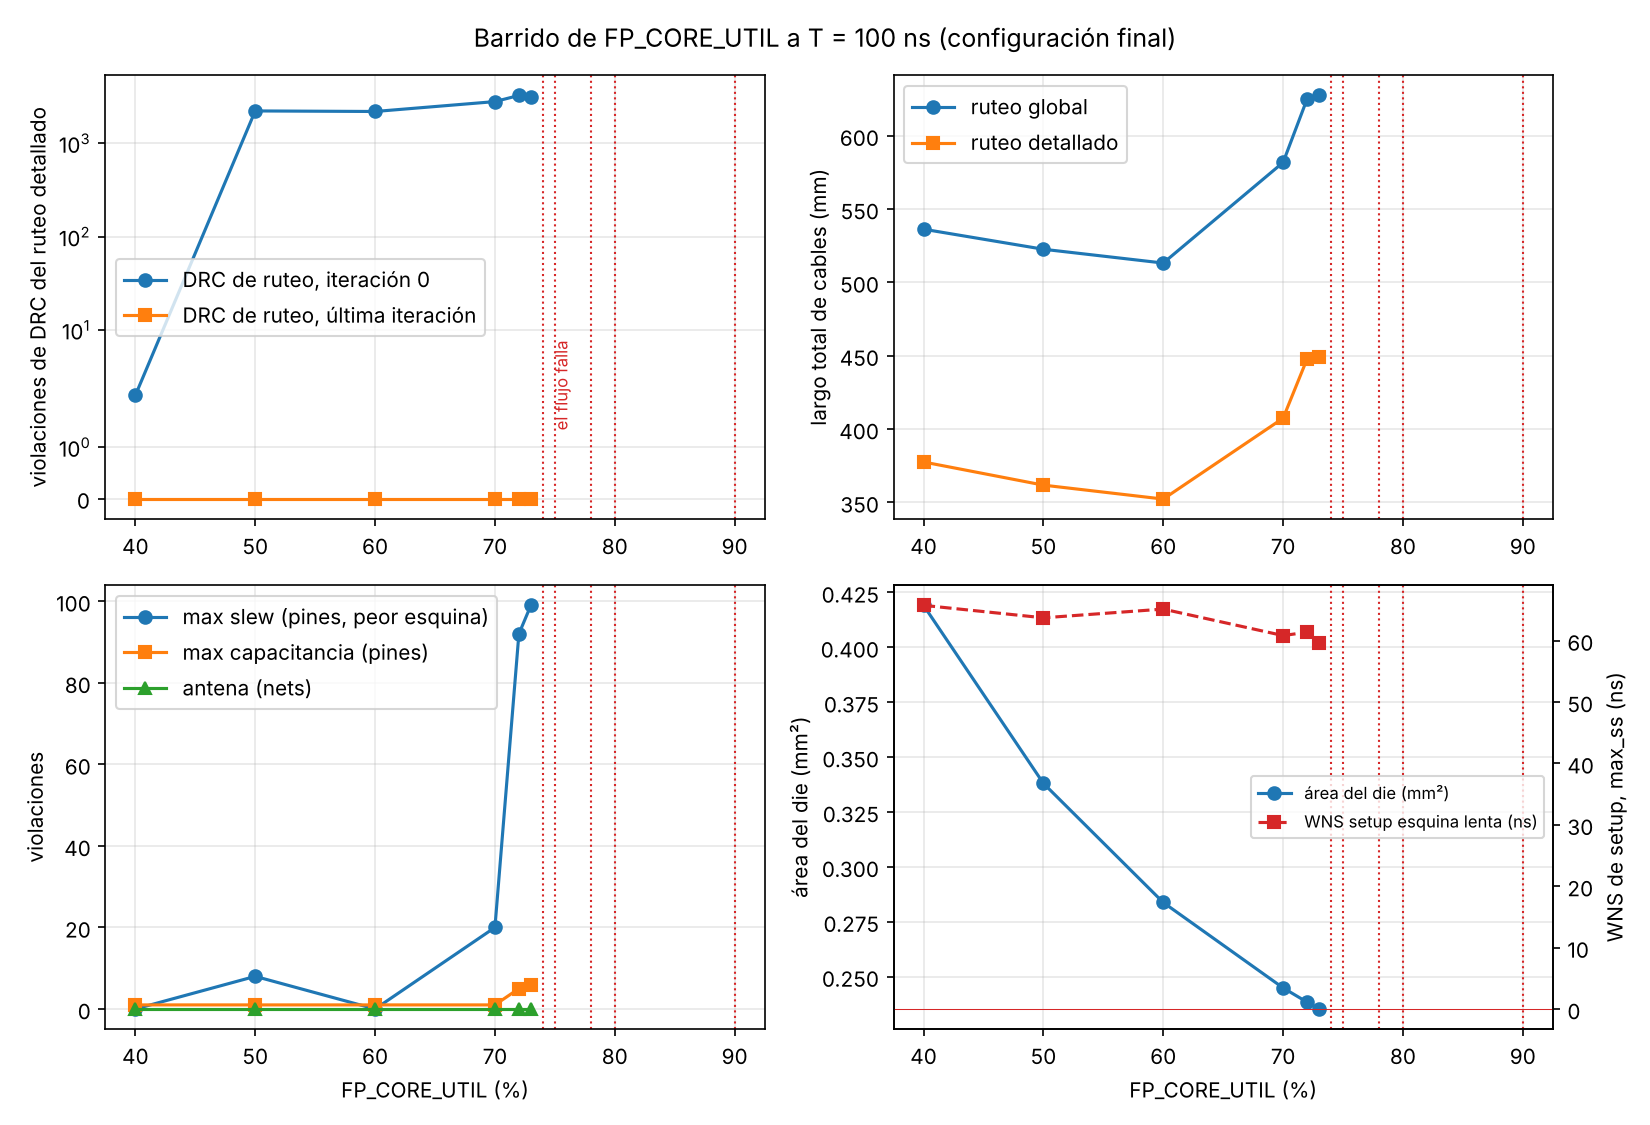
\includegraphics[width=0.92\textwidth]{../docs/figuras/utilizacion.png}
\caption{Utilización pedida contra violaciones de DRC del ruteo detallado, largo de cables, violaciones de slew, capacitancia y antena, área del die y WNS. Las líneas punteadas marcan las corridas que no terminan. Fuente: \sig{asic/graficos.py}.}
\label{fig:util}
\end{figure}

Con la utilización suben las violaciones de max slew, de 0 a 40\,\% (8 a 50\,\% y 0 a 60\,\%) a 20, 92 y 99 pines a 70, 72 y 73\,\%, y las de max capacitancia de 1 a 5 y 6: con el core casi lleno la reparación ya no tiene dónde poner buffers. El largo de cables del ruteo detallado baja hasta 60\,\% (de 377,5 a 352,2\,mm) y desde ahí sube hasta 449,4\,mm a 73\,\%, aunque el die es menor, porque el router tiene que desviar cables. Las violaciones de DRC al inicio del ruteo detallado pasan de 2 a 40\,\% a entre 2\,189 y 3\,252 desde 50\,\%, y el router las lleva a cero en todas las corridas que terminan. El die mínimo (73\,\%) y el mínimo de cables (60\,\%) no coinciden: por costo conviene el primero, por calidad del ruteo el segundo.

\subsection{Terminales del macro}

Los terminales se ubicaron por función con \sig{IO\_PIN\_ORDER\_CFG} (\sig{asic/rom/pines.cfg}, D21), como se ve en el borde de la Figura~\ref{fig:bloques}. Al oeste van las entradas: \sig{btn[3:0]}, \sig{clk} al centro del lado y \sig{rst\_n}. Al este van los dos displays, cada bus contiguo y en orden de bits; al norte los LEDs y al sur el SPI. Cada grupo llegaría así a pads vecinos de un chip completo sin cruzarse, y las señales entran por un lado y salen por el opuesto. Con la corrida final anterior se dejó que el flujo los ubicara (corrida \sig{u1\_auto}): puso \sig{clk} cerca de una esquina, llevó los botones al sur junto a tres de los cuatro terminales de SPI, juntó los LEDs con los displays en el lado este y desordenó los bits dentro de cada bus, y ahorró solo 0,4\,\% de cable con el mismo WNS.

Estos terminales son rectángulos de Metal3 (oeste y este) y Metal2 (norte y sur) en el borde del macro, y solo conectan lógica. Un chip completo rodearía el macro con un anillo de pads de I/O: celdas grandes con protección contra descargas electrostáticas, buffers de salida capaces de entregar la corriente de un LED o un display, y entradas con histéresis.

\subsection{Costo}
\label{sec:costo}

Con US\$23\,000 por mm$^2$ y un costo proporcional al área del die, la corrida final (0,419\mmd) costaría US\$9\,640, la de 73\,\% de utilización (0,235\mmd) US\$5\,410 y la estrategia 2 (1,802\mmd) US\$41\,437. La aproximación ignora que un prototipo se paga por cupo en una oblea multiproyecto con un área mínima, que el macro no incluye pads, anillo de sello ni encapsulado, que el precio por mm$^2$ baja con el volumen y que las máscaras son un costo fijo. Tampoco considera el rendimiento de fabricación, que baja con el área, así que el costo real por chip crece más rápido que el área.

La decisión con más impacto en área y costo fue la estrategia de memoria: con el mismo RTL y la misma configuración, la estrategia 2 necesita un die 4,3 veces mayor (Tabla~\ref{tab:estrategias}). La siguiente es la utilización, que de 40 a 73\,\% reduce el die en 43,9\,\%. Los cambios de D23 suben el área de celdas 14,4\,\% (de 182\,265 a 208\,439\umd: 2,3\,\% el pipeline con B2 y 11,8\,\% el modelo de cable), pero el die crece solo 2,5\,\% (de 0,409 a 0,419\mmd, US\$234 más). \sig{FP\_CORE\_UTIL} dimensiona el die sobre el área de síntesis, que sube 2,6\,\% con el pipeline, y los buffers que agrega el resizer caben adentro: el modelo de cable solo sube la utilización real, de 47,9 a 53,5\,\%.

%=====================================================================
\section{Signoff y layout}
\label{sec:signoff}
%=====================================================================

\subsection{DRC, LVS y antenas}

La corrida final no tiene violaciones de DRC (Magic), diferencias de LVS ni nets con violación de antena, y el flujo insertó un diodo de antena (Tabla~\ref{tab:cierre}). Además se corrió sobre el GDS final el deck de DRC de KLayout de GlobalFoundries (684 reglas, \sig{asic/drc/}), que LibreLane salta con este PDK, y no marcó nada. Para comprobar que el deck detecta errores, se agregaron a una copia del GDS dos violaciones de Metal1: un trazo de 0,20\um de ancho y dos trazos separados por 0,15\um, contra mínimos de 0,23\um. El deck marcó exactamente esas dos, en las reglas M1.1 y M1.2a y en sus coordenadas (\sig{asic/rom/resultados/final/drc\_klayout/control\_positivo.md}).

Durante la comparación de estrategias, antes del pipeline, apareció una violación de antena en la estrategia 2, en todas sus corridas. En \sig{s2\_t100}, el net \sig{net3342} reparte una señal de alto fanout entre cinco buffers y ocupa una envolvente de $666 \times 364$\um (Figura~\ref{fig:antena}). En el pin \sig{fanout3341/I}, la razón entre el área lateral del Metal2 conectado (perímetro por espesor) y el área de la compuerta es 449,1, 1,12 veces el máximo de 400 (\sig{asic/ff/resultados/s2\_t100/antenna.rpt}). Durante la fabricación, un tramo largo de metal conectado solo a compuertas acumula carga del grabado por plasma, y puede romper el óxido de la compuerta antes de que las capas superiores lo conecten a una difusión que la descargue.

\begin{figure}[!htb]
\centering
\begin{minipage}{0.37\textwidth}\centering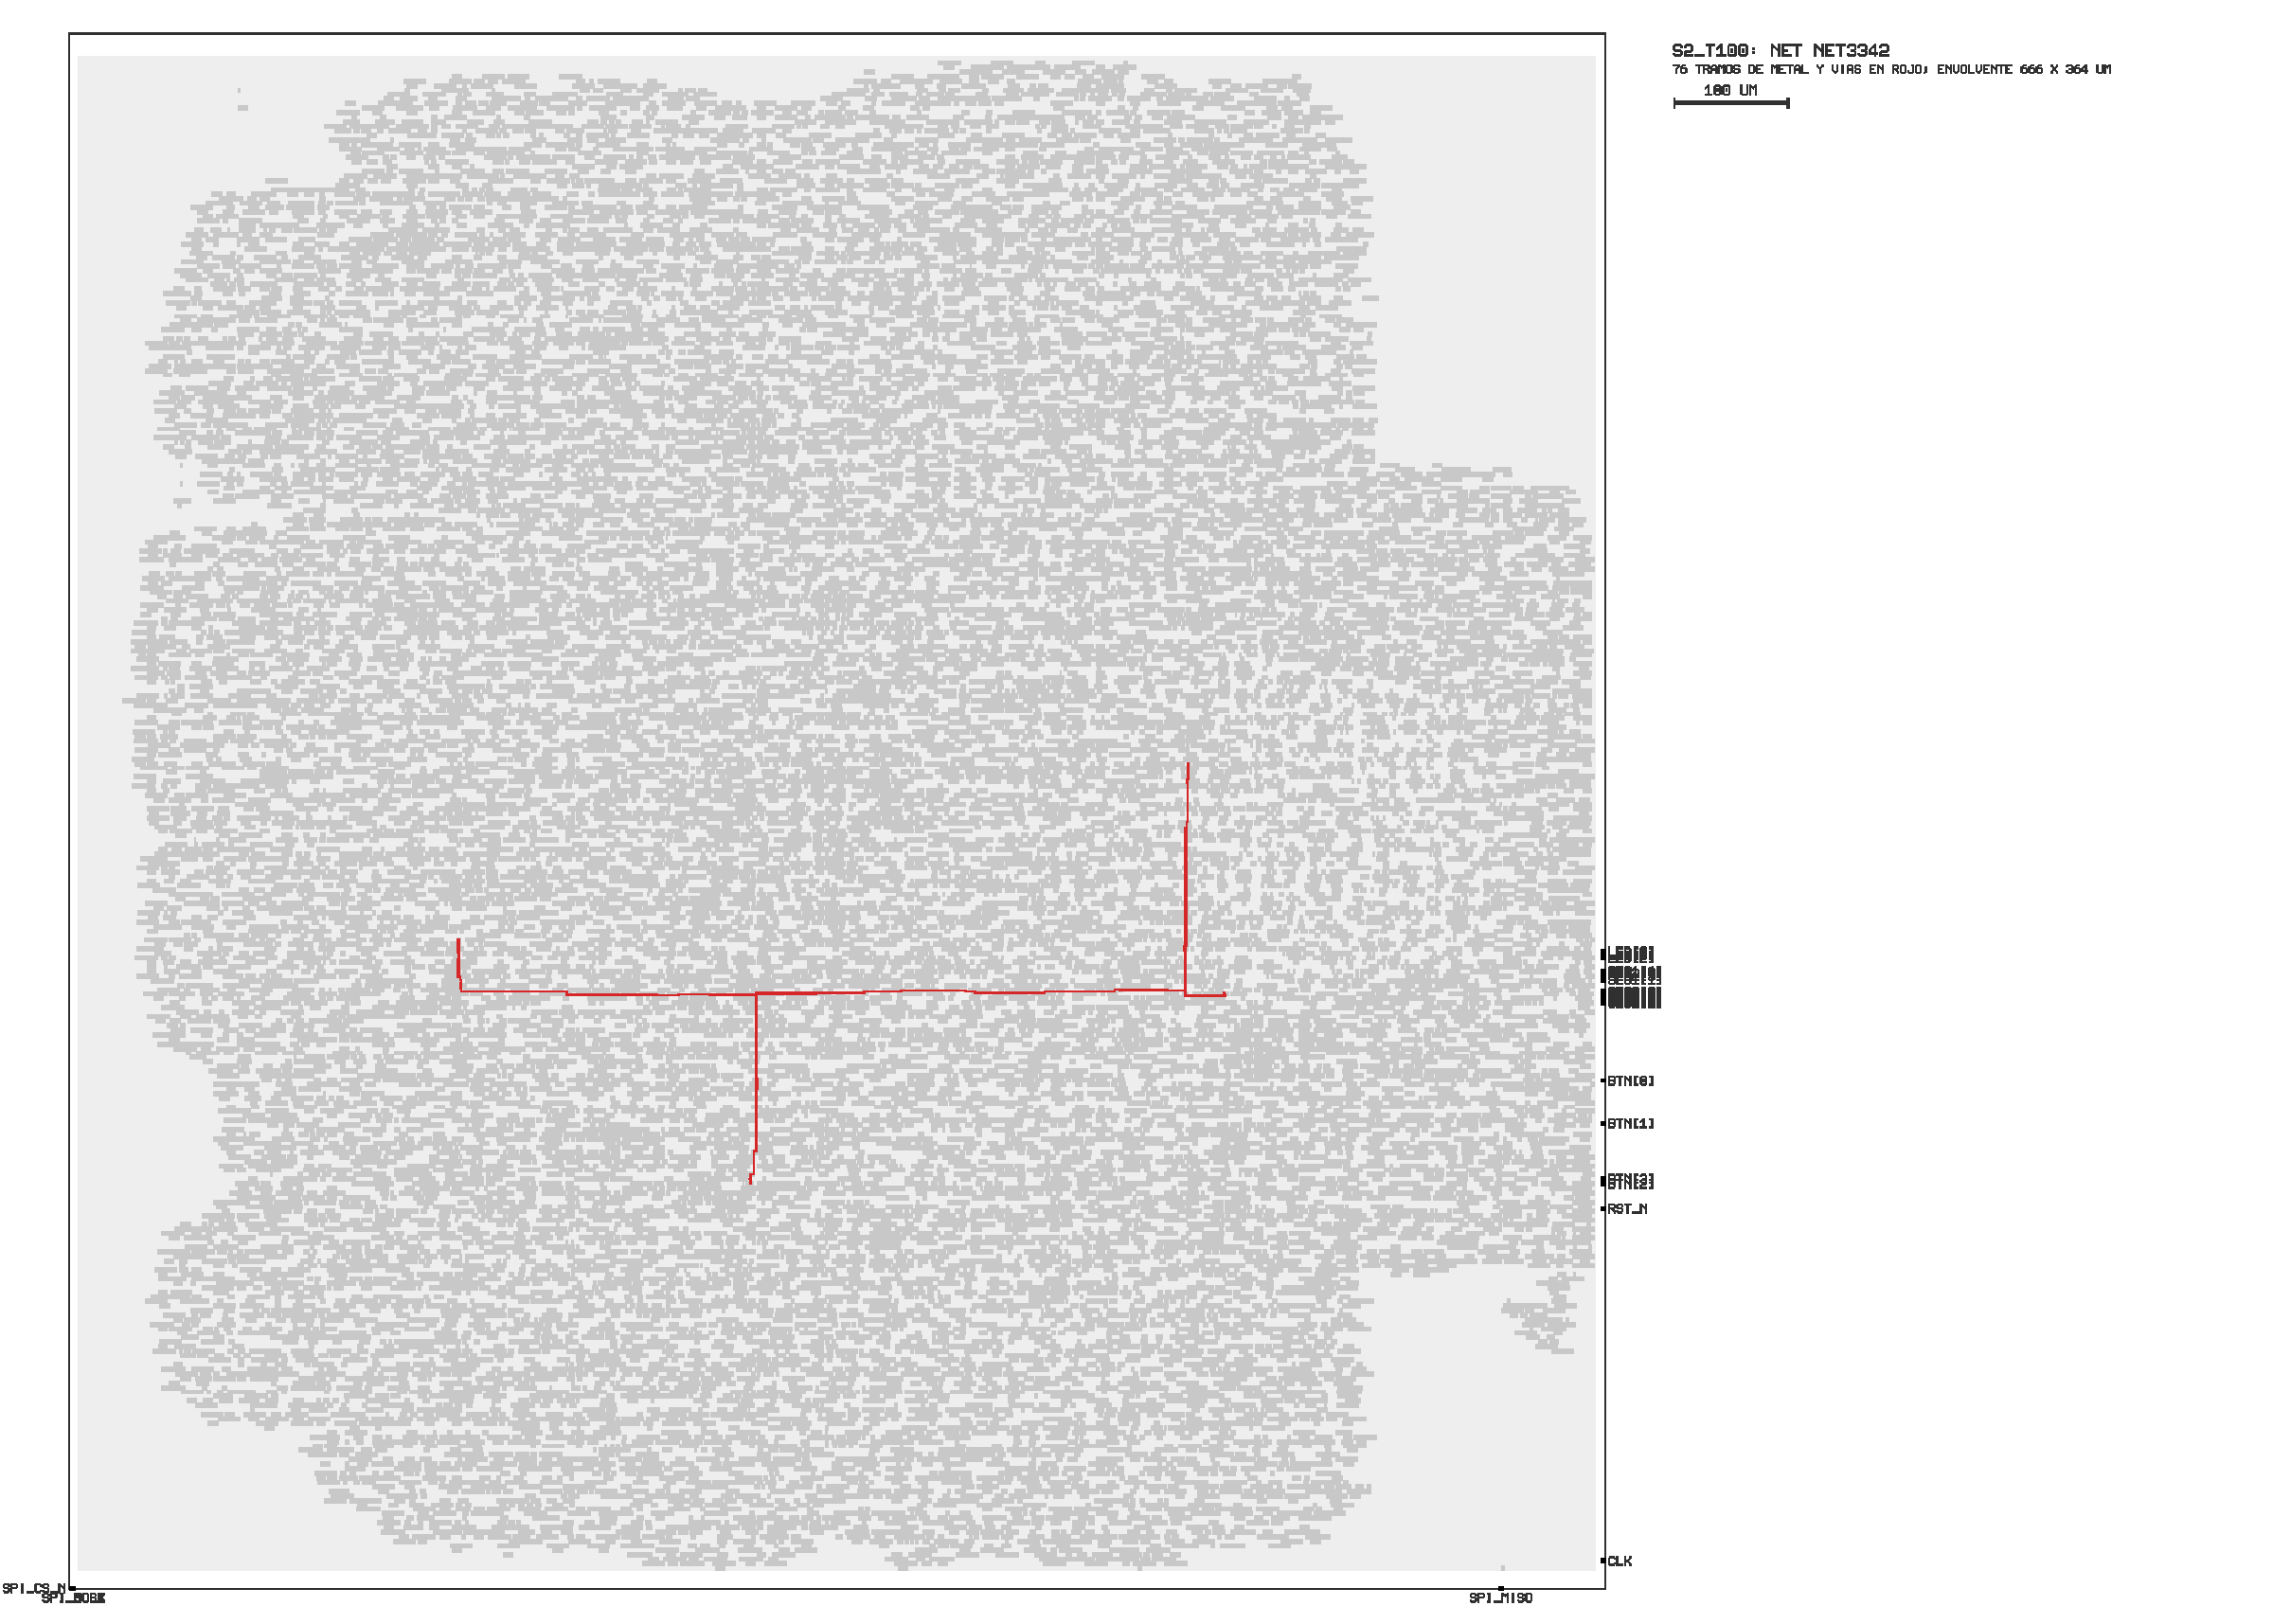
\includegraphics[width=\textwidth,trim=0 0 620 0,clip]{../asic/ff/resultados/s2_t100/layout/antena_antes.png}\end{minipage}\hfill
\begin{minipage}{0.52\textwidth}\centering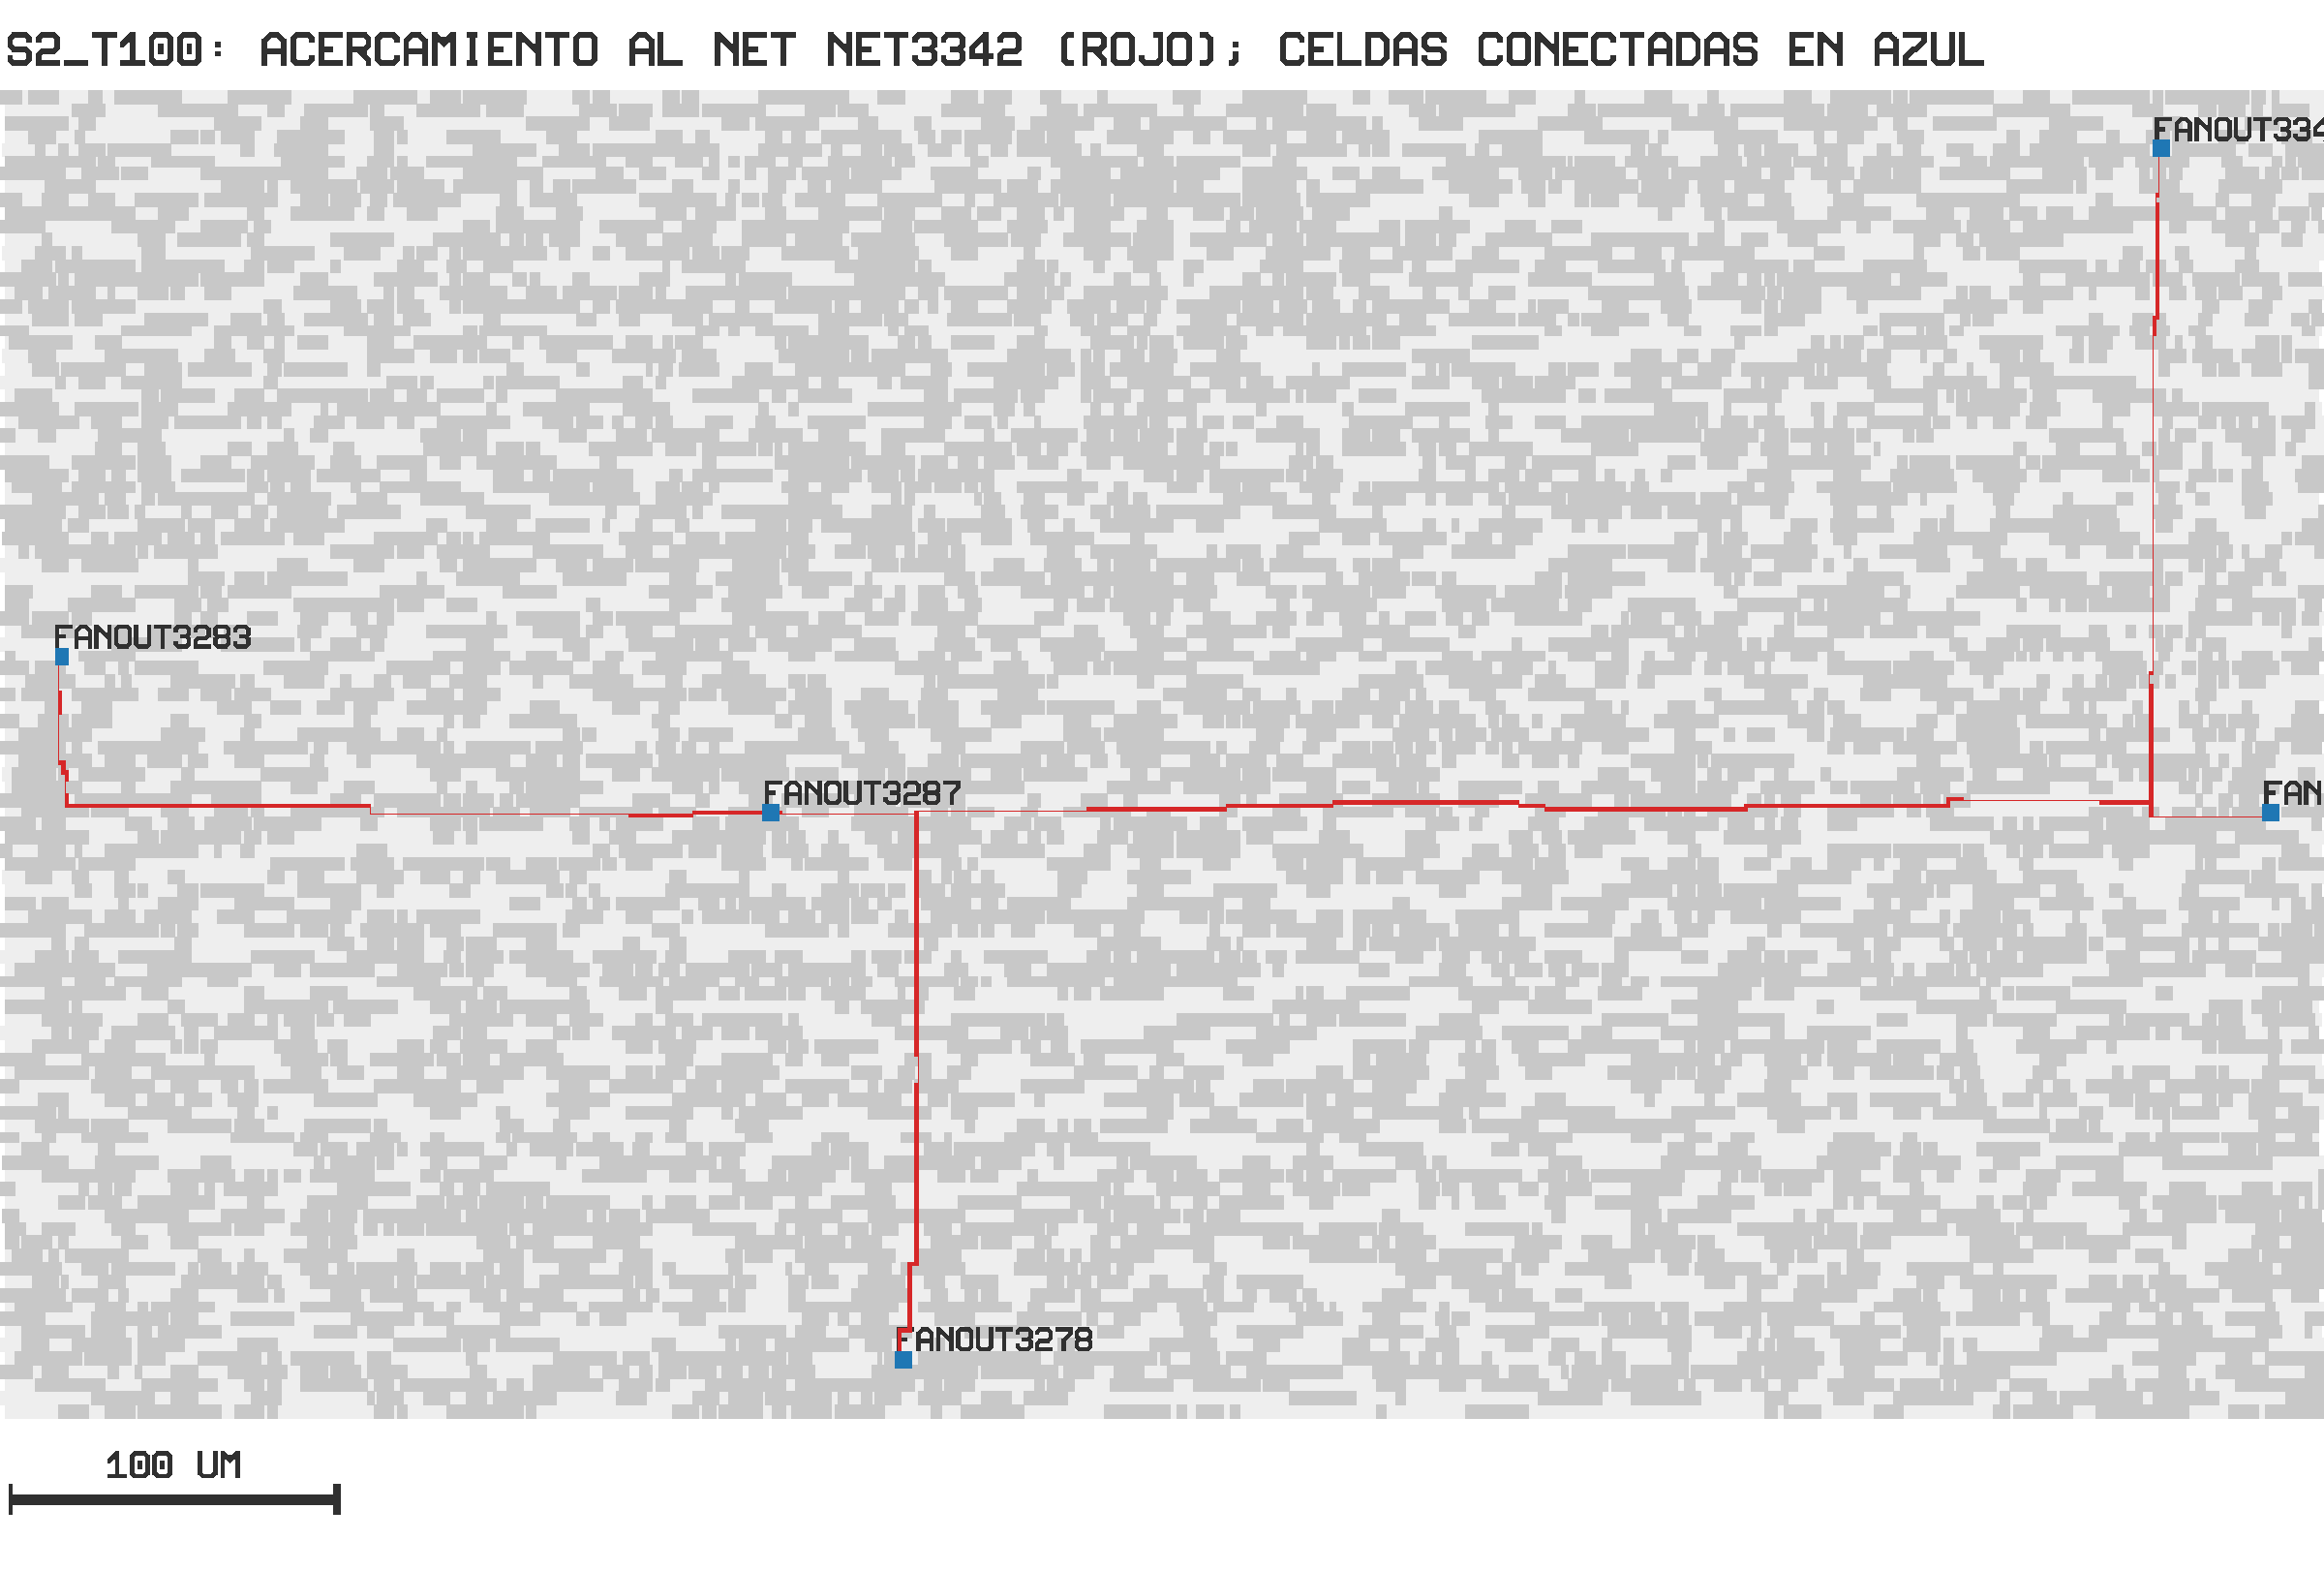
\includegraphics[width=\textwidth]{../asic/ff/resultados/s2_t100/layout/antena_antes_zoom.png}\end{minipage}
\caption{Net \sig{net3342} de \sig{s2\_t100} (rojo) sobre el layout de la estrategia 2, completo y en acercamiento, con los buffers que conecta en azul. Fuente: \sig{asic/layout/anotar.py}.}
\label{fig:antena}
\end{figure}

Se probaron dos soluciones (Tabla~\ref{tab:antena}). La inserción heurística de diodos (\sig{RUN\_HEURISTIC\_DIODE\_INSERTION}) elimina la violación pero inserta 36\,385 diodos, con 18\,\% más área de celdas y 16\,ns menos de slack. Darle más iteraciones y margen a la reparación de antenas del ruteo global (\sig{GRT\_ANTENNA\_REPAIR\_ITERS = 6}, \sig{GRT\_ANTENNA\_REPAIR\_MARGIN = 30}) también la elimina, con 108 diodos más y sin aumentar el área. Con el core y la configuración de la corrida final, la estrategia 2 ya no tiene la violación (\sig{s4\_t100}: 0 nets en violación), y la estrategia 1 no la tuvo en ninguna corrida.

\begin{table}[!htb]
\centering\small
\begin{tabular}{@{}lrrrr@{}}
\toprule
\textbf{Corrida} & \textbf{Violaciones} & \textbf{Diodos} & \textbf{Área de celdas (\textmu m$^2$)} & \textbf{WNS (ns)} \\
\midrule
\sig{s2\_t100} (original) & 1 & 150 & 838\,173 & 39,65 \\
\sig{s2\_t100\_diodos} & 0 & 36\,385 & 992\,171 & 23,65 \\
\sig{s2\_t100\_antrep} & 0 & 258 & 833\,559 & 30,03 \\
\bottomrule
\end{tabular}
\caption{Violación de antena de la estrategia 2 con el RTL anterior al pipeline y sus dos soluciones: nets con violación, celdas de antena, área de celdas y WNS de setup en \sig{max\_ss\_125C\_4v50}. Fuente: \sig{metrics.json} y \sig{antenna\_summary.rpt} de cada corrida en \sig{asic/ff/resultados/}.}
\label{tab:antena}
\end{table}

\subsection{Layout anotado}

El register file, la ALU y el contador de ciclos conservan su jerarquía en la síntesis (Sección~\ref{sec:sintesis}), así que sus celdas llegan al DEF final con el nombre de su instancia como prefijo: \sig{u\_soc.u\_core.u\_rf/}, \sig{u\_soc.u\_core.u\_id.u\_alu/} y \sig{u\_soc.u\_periph.u\_cycles/}. Un script de KLayout (\sig{asic/layout/anotar.py}) lee el DEF con los LEF del PDK, colorea las celdas de cada prefijo y genera la Figura~\ref{fig:bloques} y una base de marcadores (\sig{bloques.lyrdb}) para repetir las marcas en la interfaz de KLayout (\sig{docs/layout.md}).

\begin{figure}[!htb]
\centering
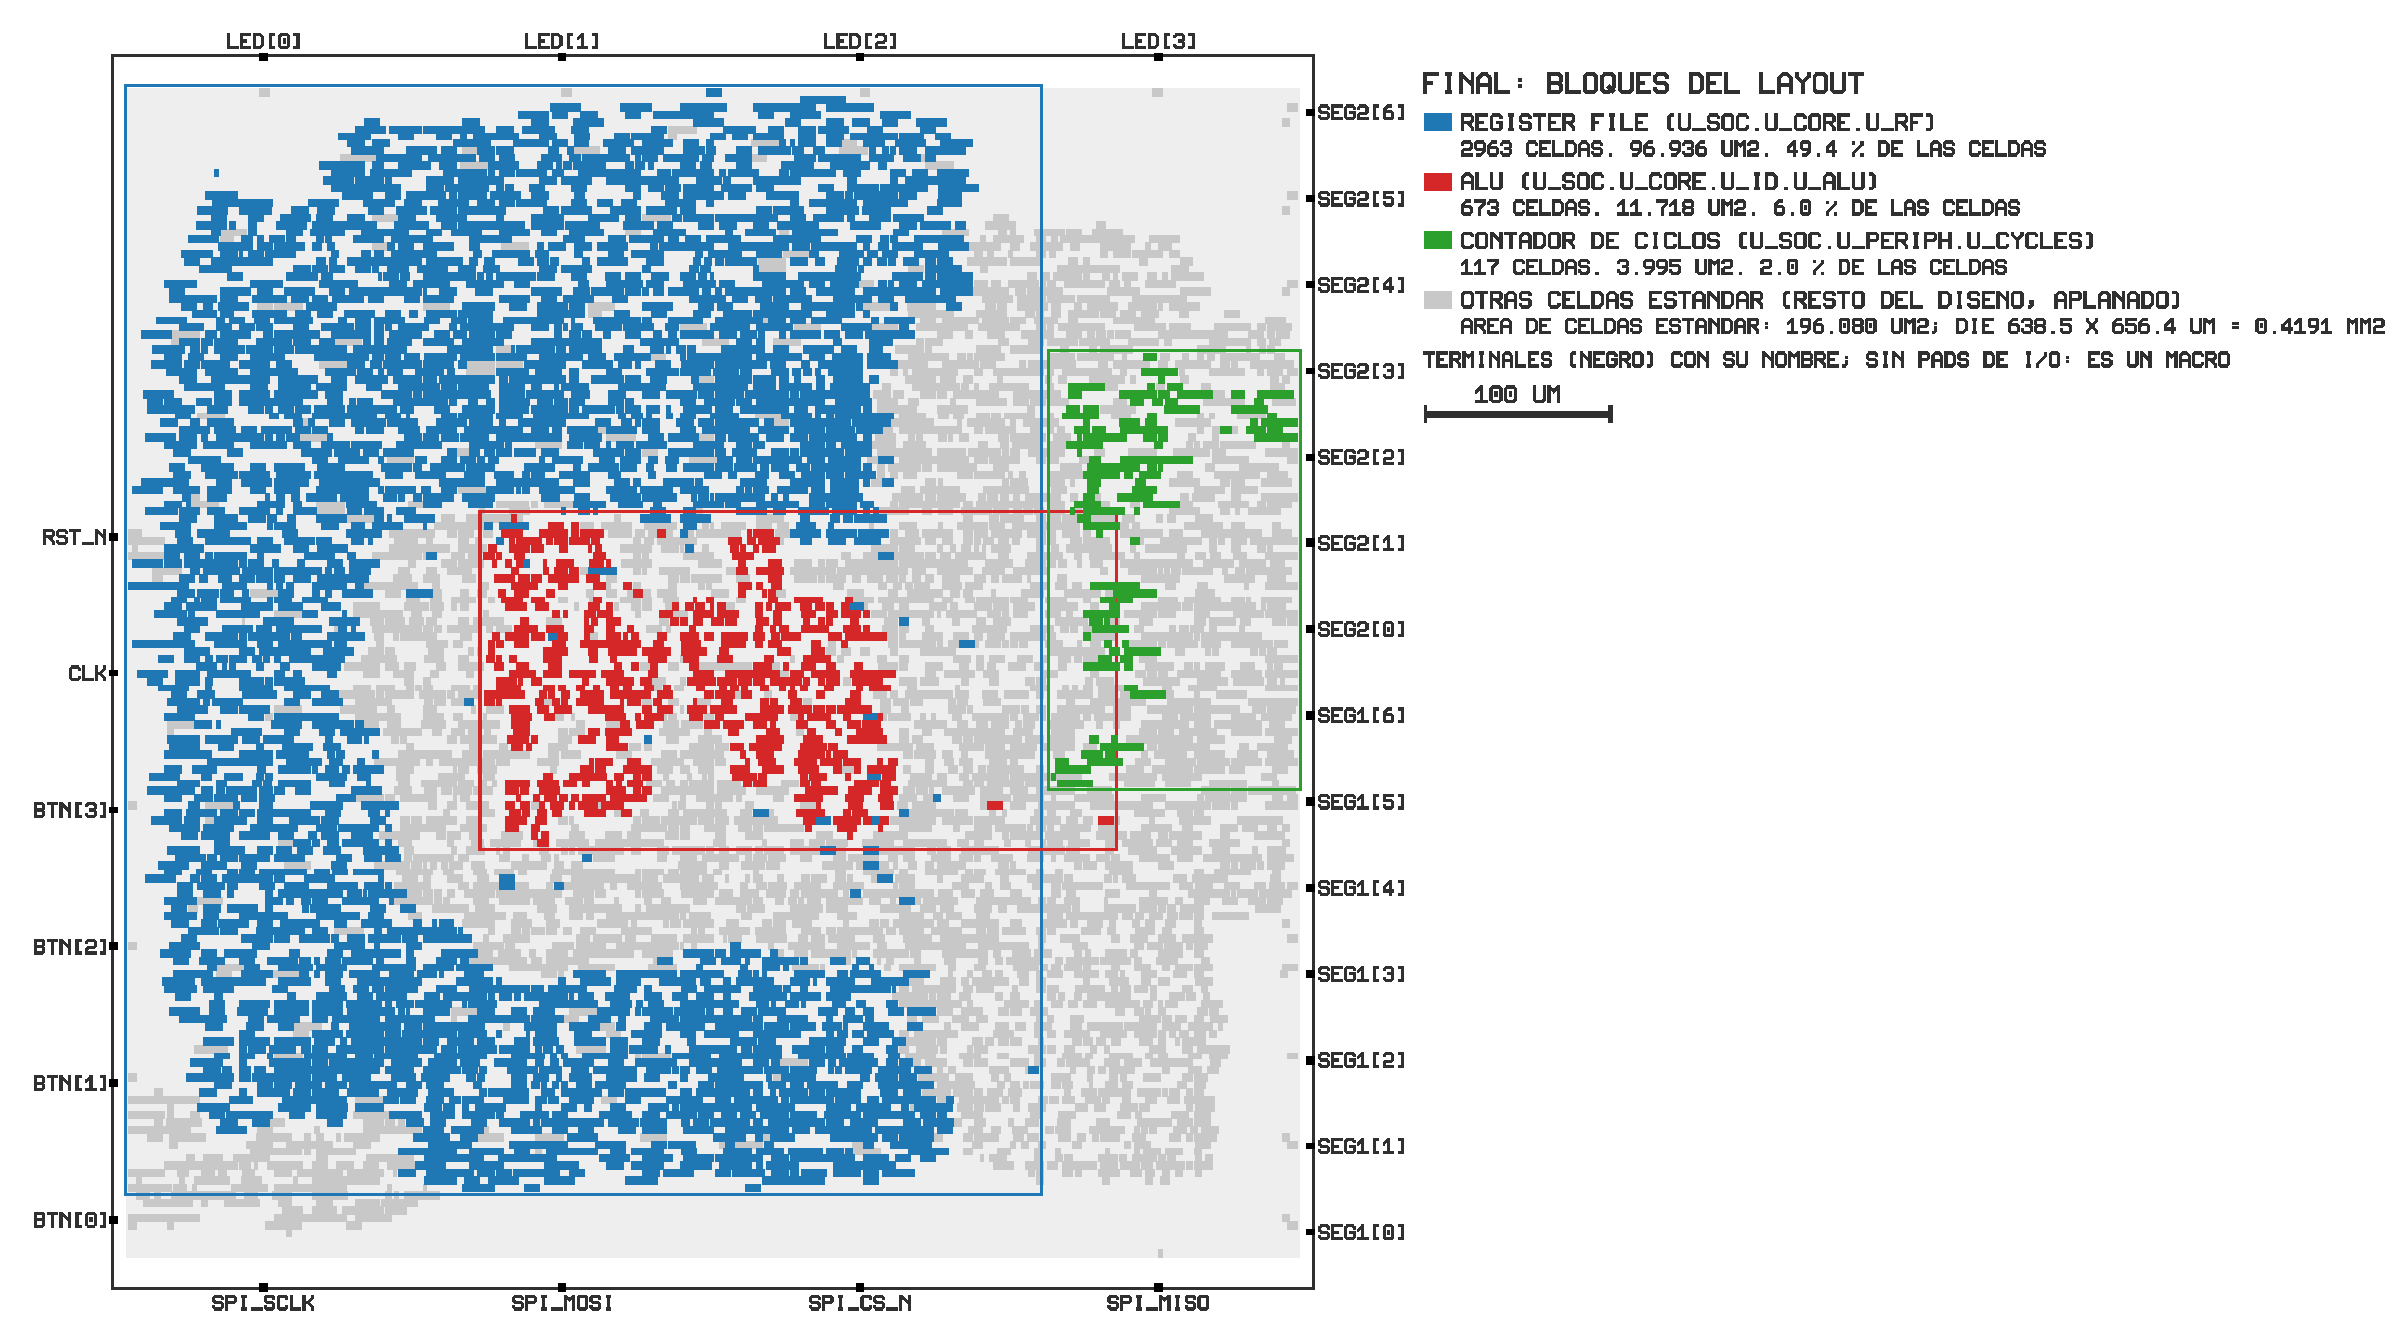
\includegraphics[width=0.9\textwidth]{../asic/rom/resultados/final/layout/bloques.png}
\caption{Layout de la corrida final con el register file (azul), la ALU (rojo) y el contador de ciclos (verde), cada uno con su rectángulo envolvente, y los terminales en el borde. Fuente: \sig{asic/rom/resultados/final/layout/}.}
\label{fig:bloques}
\end{figure}

El register file se reparte en una herradura que ocupa el oeste del core y sus franjas norte y sur, alrededor de la ALU, que queda al centro; el contador de ciclos queda en una franja cerca del borde este. Las áreas de la figura son mayores que las de síntesis (96\,936 contra 80\,349\umd en el register file) porque el resizer agrega buffers dentro de cada módulo, y sus porcentajes son sobre 196\,080\umd de celdas lógicas, sin las de tap ni las de borde.

%=====================================================================
\section{Simulación funcional post-síntesis}
\label{sec:sim}
%=====================================================================

\sig{make post-synth} simula el RTL y el netlist de celdas estándar con el mismo testbench y los mismos estímulos, y compara las trazas. El netlist sale de Yosys con la configuración final (\sig{asic/sim/config.yaml}, que solo cambia la ROM y el debounce), y las celdas se simulan con los modelos Verilog del PDK compilados sin bloques \sig{specify} (\sig{-DFUNCTIONAL}), o sea sin retardos. El testbench (\sig{tb/post\_synth\_tb.v}) usa solo los puertos de \sig{asic\_top}, aprieta los botones en ciclos absolutos leídos de \sig{asic/sim/estimulos.txt} y escribe una línea por cada cambio de los LEDs o del display.

Para que la simulación dure miles de ciclos y no millones, las dos usan el mismo \sig{game.s} ensamblado con \sig{-D CYCLES\_PER\_TENTH=1}, con lo que el display muestra directamente los ciclos medidos, y el debounce con \sig{DebounceDivBits = 2}, que acepta un botón en unos 12 ciclos (\sig{asic/sim/README.md}). El LED objetivo de cada ronda lo elige el LFSR del programa, así que los estímulos se calibraron corriendo el RTL por etapas y leyendo en su traza qué LED se encendió y cuándo (\sig{asic/sim/calibrar.py}). Cada pulsación llega 20 ciclos después de encenderse el LED y dura 60.

\begin{table}[!htb]
\centering\small
\begin{tabular}{@{}rlp{9.8cm}r@{}}
\toprule
\textbf{Ciclos} & \textbf{Botón} & \textbf{Qué pasa} & \textbf{Ciclo} \\
\midrule
300 a 360 & \sig{0001} & Pulsación de inicio; empieza la ronda 01 & 404 \\
635 a 695 & \sig{0010} & Ronda 01, LED \sig{0010}: acierto, el display muestra 51 & 1\,033 \\
1\,373 a 1\,433 & \sig{0010} & Ronda 02, LED \sig{0001}: botón incorrecto, el display muestra EE & 1\,405 \\
 & & La ronda vuelve a 02, no avanza & 1\,507 \\
1\,733 a 1\,793 & \sig{0001} & Reintento de la ronda 02: acierto, el display muestra 51 & 2\,131 \\
\bottomrule
\end{tabular}
\caption{Escenario simulado. La última columna es el ciclo en que aparece cada resultado, igual en el RTL y en el netlist. Fuente: \sig{asic/sim/resultado.md}.}
\label{tab:sim}
\end{table}

Las dos trazas son idénticas, con 17 líneas (la inicial y 16 cambios de salida) en 4\,500 ciclos y ningún valor desconocido (X) en las salidas del netlist. La ronda correcta mide 51 ciclos en las dos simulaciones, y la pulsación incorrecta muestra EE y repite la ronda 02 en vez de pasar a la 03 (Tabla~\ref{tab:sim}). Como control negativo, \sig{make post-synth-control} atrasa 8 ciclos la pulsación de la ronda 01 solo en el netlist: el display muestra 59 en vez de 51 y la comparación da FAIL. Con 7 ciclos de atraso la traza no cambia, porque el programa lee los botones en un lazo de 8 ciclos y la medición no distingue pulsaciones dentro de la misma vuelta. Con las constantes reales, el netlist de la corrida final también coincide con el RTL durante 320\,000 ciclos, hasta los cuatro LEDs y el 01 de la primera ronda, en los ciclos 262\,151 y 262\,172 (\sig{make post-synth-final}). Además, el flujo de equivalencia formal de Yosys prueba que el RTL es equivalente a los netlists de síntesis y post-PnR (976 de 976 y 968 de 968 celdas \sig{\$equiv}, \sig{docs/equivalencia.md}).

La simulación opcional con retardos usa el netlist y el SDF de una corrida completa con la configuración de simulación (\sig{d2\_pnr}, que cierra) y el mismo escenario, en las esquinas típica, lenta y rápida, con tres ejecuciones por esquina en dos simuladores. Icarus Verilog 13.0 anota los retardos pero no evalúa los timing checks; Open Verilog CVC 7.00b sí evalúa los 7\,173 checks del SDF (\sig{\$setup}, \sig{\$hold}, \sig{\$width}, \sig{\$recovery}, \sig{\$removal} y \sig{\$period}). Las 18 trazas son idénticas a la del RTL, sin valores X, y CVC no reporta ninguna violación. Como control, aplicar las entradas 1\,ns después del flanco produce 8 violaciones en los cuatro flip-flops que reciben una señal externa que cambia en el escenario (los dos del sincronizador de reset y los de los botones 0 y 1), porque el reloj les llega unos 1,4\,ns después del flanco externo; por eso el escenario con SDF aplica las entradas a mitad de ciclo. El netlist de la corrida final con su SDF de la esquina típica también reproduce al ciclo los 320\,000 ciclos del escenario con las constantes reales (\sig{asic/sim/resultado\_sdf.md}).

\end{document}
